

%% AP Physics MC Questions Archive
%%----------------------------------------


%% Two Dimensional Motion with Vecotrs
%%----------------------------------------
\element{ap}{
\begin{question}{2d-motion-vectors-q01}
    A ship travels 5 miles due east and then 12 miles due north.
    What is the net displacement of the ship?
    \begin{multicols}{2}
    \begin{choices}
        \wrongchoice{7 miles}
      \correctchoice{13 miles}
        \wrongchoice{16 miles}
        \wrongchoice{17 miles}
        \wrongchoice{19 miles}
    \end{choices}
    \end{multicols}
\end{question}
}

\element{ap}{
\begin{question}{2d-motion-vectors-q02}
    In still water a ship can produce a maximum velocity of \SI{5}{\meter\per\second} in any direction.
    This same ship is placed in a river with a current of \SI{5}{\meter\per\second} eastward.
    \begin{center}
    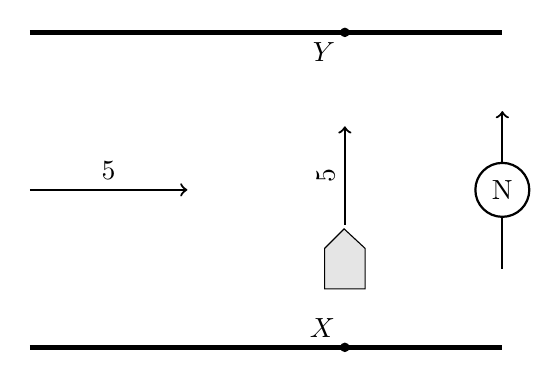
\begin{tikzpicture}
        %% Banks
        \draw[ultra thick] (-3,-2) -- (+3,-2);
        \draw[ultra thick] (-3,+2) -- (+3,+2);
        %% north
        \draw[thick,->] (+3,-1)  -- (+3,1) node[pos=0.5,anchor=center,draw,thick,circle,fill=white] {N};
        %% Boat
        \node[minimum size=0.5cm] (B) at (+1,-1) {};
        \draw[fill=white!90!black] (B.north west) -- ++(45:0.35) -- (B.north east) -- (B.south east) -- (B.south west) --cycle;
        \draw[thick,->] (B.north) ++(90:0.3) -- ++(90:1.25) node[pos=0.5,anchor=south,rotate=90] {\SI{5}{\meter\per\second}};
        %% Current
        \draw[thick,->] (-3,0) -- (-1,0) node[pos=0.5,anchor=south] {\SI{5}{\meter\per\second}};
        %% Point X and Y
        \draw [fill] (1,-2) circle (1.5pt) node[anchor=south east] {$X$};
        \draw [fill] (1,+2) circle (1.5pt) node[anchor=north east] {$Y$};
    \end{tikzpicture}
    \end{center}
    With what velocity should the boat be operated with in order to reach point $Y$ from point $X$?
    (Note: Point $Y$ is due north of point $X$)
    \begin{choices}
        \wrongchoice{\SI{5}{\meter\per\second} due West until the ship is far enough out, then \SI{5}{\meter\per\second} due North.}
        \wrongchoice{Simultaneously, \SI{2.5}{\meter\per\second} due West and \SI{2.5}{\meter\per\second} due North.}
        \wrongchoice{\SI{5}{\meter\per\second} due North.}
        \wrongchoice{\SI{5}{\meter\per\second} due North until the ship has reached the northern shore. Then \SI{5}{\meter\per\second} due West until the ship reaches point $Y$.}
      \correctchoice{The ship's engine is not powerful enough to reach point $Y$.}
    \end{choices}
\end{question}
}

\element{ap}{
\begin{question}{2d-motion-vectors-q03}
    A ship can travel at a maximum speed of \SI{8}{\kilo\meter\per\hour} in any direction in still water.
    What is the maximum velocity of the ship relative to the shore if it is moving perpendicular to a \SI{6}{\kilo\meter\per\hour} current?
    \begin{multicols}{3}
    \begin{choices}
        \wrongchoice{\SI{4}{\kilo\meter\per\hour}}
        \wrongchoice{\SI{6}{\kilo\meter\per\hour}}
        \wrongchoice{\SI{8}{\kilo\meter\per\hour}}
        \wrongchoice{\SI{9}{\kilo\meter\per\hour}}
      \correctchoice{\SI{10}{\kilo\meter\per\hour}}
    \end{choices}
    \end{multicols}
\end{question}
}

\element{ap}{
\begin{question}{2d-motion-vectors-q04}
    A truck traveled \SI{1200}{\meter} south in \SI{80}{\second} and then \SI{500}{\meter} west in \SI{20}{\second}.
    The magnitude of the average velocity of the truck is most nearly:
    \begin{multicols}{3}
    \begin{choices}
        \wrongchoice{\SI{10}{\meter\per\second}}
      \correctchoice{\SI{13}{\meter\per\second}}
        \wrongchoice{\SI{17}{\meter\per\second}}
        \wrongchoice{\SI{25}{\meter\per\second}}
        \wrongchoice{\SI{30}{\meter\per\second}}
    \end{choices}
    \end{multicols}
\end{question}
}

\element{ap}{
\begin{question}{2d-motion-vectors-q05}
    A car, starting from rest,
        experiences a constant acceleration for \SI{5}{\second} such that it moves \SI{200}{\meter} west and \SI{150}{\meter} north.
    What was the magnitude of this acceleration?
    \begin{multicols}{3}
    \begin{choices}
        \wrongchoice{\SI{5}{\meter\per\second\squared}}
        \wrongchoice{\SI{10}{\meter\per\second\squared}}
      \correctchoice{\SI{20}{\meter\per\second\squared}}
        \wrongchoice{\SI{40}{\meter\per\second\squared}}
        \wrongchoice{\SI{100}{\meter\per\second\squared}}
    \end{choices}
    \end{multicols}
\end{question}
}


\endinput


